% =====================================================================
%  Strong Optical Disorder Erases Images but Preserves Local Change
%  Observability  --  PRL Letter (Rank-Jet Separation)
%  Binding spec: docs/ROUND63_GPT_ROUND43_RULING_RAW.md
%  Every numerical claim traces to paper_prl/CLAIM_SOURCE_MATRIX.md.
%  American spelling. PRL Letter: unnumbered headings; End Matter A/B/C.
% =====================================================================
\documentclass[aps,prl,reprint,groupedaddress,superscriptaddress,floatfix]{revtex4-2}

\usepackage{graphicx}
\usepackage{amsmath}
\usepackage{amssymb}
\usepackage{bm}
\graphicspath{{figures/}}

\newcommand{\Treq}{T_{\mathrm{req}}}
\newcommand{\Cstar}{C_{\ast}}
\newcommand{\tr}{\operatorname{tr}}
\newcommand{\rank}{\operatorname{rank}}
\newcommand{\eps}{\varepsilon}

\begin{document}

\title{Strong Optical Disorder Erases Images but Preserves Local Change Observability}

\author{[AUTHORS]}
\affiliation{[AFFILIATION]}

\date{\today}

\begin{abstract}
Strong disorder is expected to erase spatial information. We show that
reconstruction rank and local change observability are distinct invariants.
After nuisance profiling, the first nonzero Chernoff jet of a perturbation
fixes its detection-time exponent. In an amplitude-anchored scrambled channel
the scene Fisher matrix collapses to rank one, yet every nonzero local change
stays visible: generic directions need $T\!\sim\!\eps^{-2}$, first-order-orthogonal
ones are curvature-rescued at $T\!\sim\!\eps^{-4}$. Exact divergences, Monte Carlo, sequential detection,
and a sealed bucket-optics test validate the result.
\end{abstract}

\maketitle

% ---------------------------------------------------------------------
% OPENING: the disorder paradox  (0.40 pp)
% ---------------------------------------------------------------------
\section*{The disorder paradox}
A strongly scattering medium destroys the map between an object and its image.
In the fully developed speckle limit the mean field carries only the object's
total flux, and every attempt to invert the scrambled transmission fails once
the angular memory effect is exhausted~\cite{FengMemory,Mudry}. The received
wisdom is therefore that strong disorder erases spatial information outright. We show that this conflates
two logically independent quantities. \emph{Reconstruction rank}---how many
scene coordinates a record can resolve---can collapse to one, while \emph{local
change observability}---whether an infinitesimal scene change alters the
measured statistical law at all---remains complete. The physical statement of
the Letter is that strong optical disorder can erase coordinates without erasing
the observability of local change, and that a single invariant, the order of the
first nonzero nuisance-profiled statistical jet, fixes the price of observing
each direction.

The claim is not ``detection is easier than imaging.'' It is a classification of
physical observability by contact order that survives reparameterization and
nuisance profiling, applies to any dominated statistical experiment, and is
realized at its most extreme in complete optical scrambling. We prove a
Rank--Jet Separation theorem, demonstrate its exact directional classes, and
falsify it at its own boundaries in a sealed single-pixel optical experiment.

% ---------------------------------------------------------------------
% QUOTIENT INFORMATION JETS  (0.80 pp)
% ---------------------------------------------------------------------
\section*{Quotient information jets}
Let one independent medium realization (``bank'') generate a record $Y$ with law
$P_{x,\eta}$, where $x$ is the static scene and $\eta$ collects every admitted
nuisance: the medium law, throughput, temporal, and detector degrees of freedom.
Along a physical scene path $x_\eps=x+\eps\delta$ the relevant question is not
whether a chosen observable moves, but whether the perturbed law leaves the
nuisance orbit $N_x=\{P_{x,\eta'}\}$. We therefore profile every nuisance and
work with the profiled Chernoff distance
$\Cstar(\eps;\delta)=\inf_{\eta'}C(P_{x+\eps\delta,\eta},P_{x,\eta'})$, whose
infimum makes it invariant to nuisance coordinates, gain gauges, and changes of
medium basis. If $\Cstar(\eps;\delta)=c_m(\delta)\,\eps^{2m}+o(\eps^{2m})$ with
$c_m>0$, then
%
\begin{equation}
\Treq\asymp\eps^{-2m},
\label{eq:jet}
\end{equation}
%
and we call $m=m(\delta)$ the \emph{quotient information-jet order}. For $T$
independent-equivalent banks Chernoff's theorem gives
$-T^{-1}\log P_e^{\ast}(T,\eps)\to\Cstar(\eps;\delta)$, so the fixed-error sample
complexity obeys Eq.~\eqref{eq:jet}; the same profiled
Kullback--Leibler expansion drives Lorden/CUSUM quickest detection~\cite{Lorden},
giving a mean delay $\propto\eps^{-2m}$. The quotient jet is a stochastic
observability order, the statistical counterpart of successive-derivative
observability rank conditions~\cite{HermannKrener}, and the efficient profiled
score is the unique statistic that saturates the fluctuation--response
bound~\cite{Dechant}. The exponent is a property of the physical
experiment after nuisance quotienting: it assumes no fixed trace, no isotropy,
and no chosen estimator. Physical covariation changes the coefficient $c_m$; it
cannot change the definition of $m$. This is the object that survives the
spectral covariations which defeat any fixed-resource inequality.

% ---------------------------------------------------------------------
% RANK-JET SEPARATION  (0.55 pp)
% ---------------------------------------------------------------------
\section*{Rank--Jet Separation}
Suppose the marginal record law depends on the scene through $r$ smooth
functionals $q(x)=(q_1,\dots,q_r)$, $P_x=P_{q(x),\eta}$, with every nuisance
profiled out. Writing $J_q$ for the efficient Fisher matrix in functional space,
the scene Fisher matrix factors as
%
\begin{equation}
I_x=Dq_x^{\!\top}J_q\,Dq_x,\qquad \rank(I_x)\le r .
\label{eq:rank}
\end{equation}
%
Thus $r=1$ permits at most rank-one reconstruction information, regardless of how
many detector samples are acquired. Reconstruction rank is bounded by the number
of scene functionals the law exposes; it says nothing about the contact order of
any one direction.

The strongest realization is the fully scrambled covariance channel. There a
single nonnegative scalar $Q(x)=x^{\!\top}Gx$ (a grain-weighted scene energy,
$G\succ0$) enters the record covariance, so
%
\begin{equation}
\Sigma(x)=R+Q(x)\,H,\qquad
\Delta Q = 2\,x^{\!\top}G\delta + \delta^{\!\top}G\delta .
\label{eq:Q}
\end{equation}
%
The quotient expansion of $Q$ has first variation $u(\delta)=2x^{\!\top}G\delta$
and curvature $v(\delta)=2\delta^{\!\top}G\delta>0$ for every $\delta\neq0$.
Because a regular reduced law inherits the contact order of $Q$, every direction
falls into exactly one of two local classes,
%
\begin{equation}
\begin{aligned}
x^{\!\top}G\delta\neq0 &:\; m=1,\quad \Treq\sim\eps^{-2};\\[2pt]
x^{\!\top}G\delta=0 &:\; m=2,\quad \Treq\sim\eps^{-4}.
\end{aligned}
\label{eq:classes}
\end{equation}
%
Hence \emph{the reconstruction Fisher matrix is rank one, yet the local blind set
is empty}: the first-order-orthogonal directions are not blind but
curvature-rescued, since $\delta^{\!\top}G\delta>0$. This is the Rank--Jet
Separation theorem, proved in End Matter~A.

Three boundaries fix its exact domain and make it stronger, not weaker. The
statement is \emph{local}: a signed finite change can return to the same $Q$
ellipsoid at $\eps_\ast=-2x^{\!\top}G\delta/\delta^{\!\top}G\delta$, where
distinguishability vanishes. An unanchored covariance-amplitude nuisance renders
the scene and amplitude derivatives collinear and collapses the quotient
information to zero, so a wavelength, lag-shape, polarization, or finite
calibration \emph{anchor} is required. Global sign-definiteness holds only on the
monotone cone $x,\delta\ge0$ with an entrywise-nonnegative kernel; it is not
claimed for arbitrary signed changes.

% ---------------------------------------------------------------------
% SCRAMBLING INVERSION  (0.55 pp)  + Fig 1
% ---------------------------------------------------------------------
\begin{figure*}[t]
\centering

\includegraphics[width=\textwidth]{fig1_hero.pdf}
\caption{\textbf{Rank collapses; jets survive.} As optical disorder grows from a
thin multiplicative screen to complete scrambling, the mean-channel spatial
support contracts $B_p\!\to\!\{0\}$ (DC only) and the reconstruction Fisher rank
collapses from many modes to one ($99.99\%$ of the covariance energy in the
single direction $Gx$), while the quotient jet order stays finite ($m=1$ or $2$)
and the local blind set stays empty. At the scrambling endpoint the record
covariance factors as $\mathrm{Cov}(b)=Q(x)\,(O\!\circ\!O)+R$ with
$Q=x^{\!\top}Gx$, and the two directional classes $u=2x^{\!\top}G\delta$,
$v=2\delta^{\!\top}G\delta$ set the contact order. The amplitude-anchor condition
(icon) is a prerequisite, not a caveat: without it the quotient information
vanishes.}
\label{fig:hero}
\end{figure*}

\section*{Scrambling inversion}
Complete optical scrambling supplies the extreme endpoint. A band-limited
modulator imprints a code $p_i$ (Fourier support $B_p$) on the illumination;
a dynamic strongly scattering medium with fully developed speckle then produces a
zero-mean circular-complex-Gaussian field, and a single-pixel bucket sums the
scene-weighted intensity. The mean speckle envelope is flat, so the first-moment
channel measures only the scene DC term,
%
\begin{equation}
\mathbb{E}[b_i]=C(0)\,O_{ii}\,\hat{x}(0),
\label{eq:mean}
\end{equation}
%
and its spatial support is $B_{\mathrm{mean}}=\{0\}$: every non-DC change, in-band
or beyond-band, is exactly invisible to the mean. Numerically the mean response to
a beyond-band, DC-free change has relative magnitude $6.6\times10^{-19}$.

The intensity covariance, by the Siegert relation, factors into a known code part
and the single scene scalar, $\mathrm{Cov}(b_i,b_j)=O_{ij}^2\,Q(x)$ with
$Q(x)=x^{\!\top}Gx$ and $G$ the modulus-squared grain kernel. The support of $G$
is enormous---the wavelength-scale grain pierces the modulator band---but the
scene enters through the one scalar $Q$, so the reconstruction Fisher information
is rank one and $99.99\%$ of the measured covariance energy lies in the single
direction $Gx$. Beyond-band imaging dies with the memory
effect~\cite{Idier,Chaigne}. Yet by
Eq.~\eqref{eq:Q} any beyond-band change lifts $Q$ by
$2x^{\!\top}G\delta+\delta^{\!\top}G\delta$, and the quadratic floor is strictly
positive for every nonzero $\delta$: there is no blind direction for detection.
The mean wall supplies specificity; the covariance curvature supplies detection
(Fig.~\ref{fig:hero}).

% ---------------------------------------------------------------------
% DECISIVE TESTS  (0.60 pp)  + Fig 2
% ---------------------------------------------------------------------
\begin{figure*}[t]
\centering
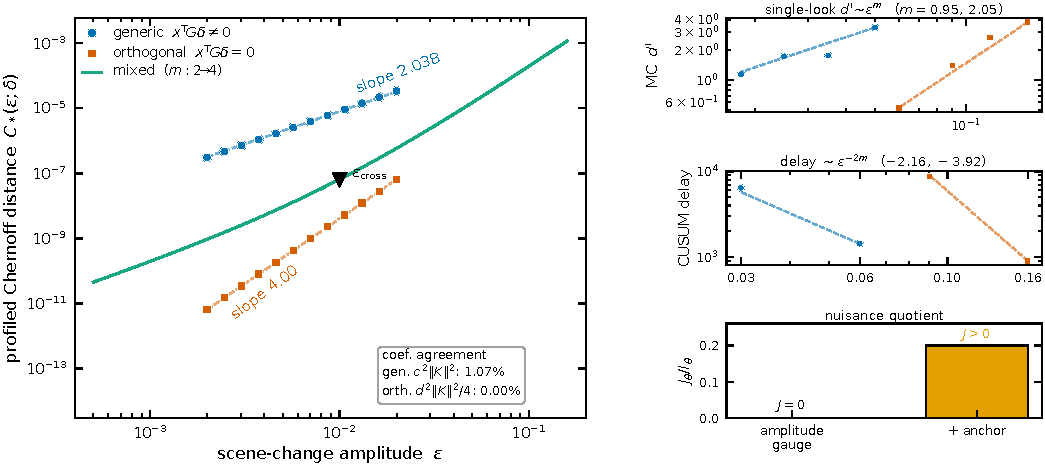
\includegraphics[width=\textwidth]{fig2_jet_slopes.pdf}
\caption{\textbf{The exponent hierarchy.} Profiled Chernoff distance versus
scene-change amplitude for a generic direction ($x^{\!\top}G\delta\neq0$,
$m=1$) and a first-order-orthogonal direction ($x^{\!\top}G\delta=0$, $m=2$),
with exact contact orders $2.038$ and $4.000$ and coefficient agreement to
$1.07\%$ and $0.00\%$ with Eq.~\eqref{eq:classes}. A mixed direction crosses over
near the predicted $\eps_{\mathrm{cross}}$. Insets: Monte Carlo single-look $d'$
exponents $0.95$ and $2.05$; CUSUM delay slopes $-2.16$ and $-3.92$; and the
nuisance quotient, which is zero under a free amplitude gauge ($J_\theta=0$) and
restored by a finite anchor ($J_\theta>0$). All sources are the committed
JET\_TEST artifact.}
\label{fig:jets}
\end{figure*}

\section*{Decisive tests}
We test the theorem with the exact scrambling generator and no reconstruction,
on a $32\times32$ grid ($N=1024$, code band $P_B=3$, grain band $K=13$, $M=36$
codes, $10^4$ photons per bucket). Directions are constructed to be generic,
exactly $G$-orthogonal, or mixed. Sweeping the amplitude over a decade and
forming exact Gaussian divergences, Monte Carlo log-likelihood-ratio error, and
CUSUM delay yields the frozen result: exact KL orders were $2.038$ and $4.000$,
Monte Carlo response exponents were $0.95$ and $2.05$, and CUSUM delay slopes
were $-2.16$ and $-3.92$; the predicted crossover, nuisance collapse, anchor
restoration, iso-$Q$ cancellation, and monotone-cone corollary all passed their
frozen tests (Fig.~\ref{fig:jets}). Under a free medium-amplitude nuisance the
efficient information for $Q$ collapses to numerical zero and stays zero across
proportional lags; a finite amplitude anchor restores it. At the signed
iso-$Q$ crossing the classifier returns to chance ($\mathrm{AUC}\approx0.48$)
while remaining visible on either side, confirming that the completeness is local.
Over $400$ in-aperture directions the blind fraction is exactly zero. All
$17$ predeclared checks passed and none of the four kill conditions fired.

% ---------------------------------------------------------------------
% SEALED OPTICAL INSTANTIATION  (0.35 pp)  + Fig 3
% ---------------------------------------------------------------------
\begin{figure*}[t]
\centering
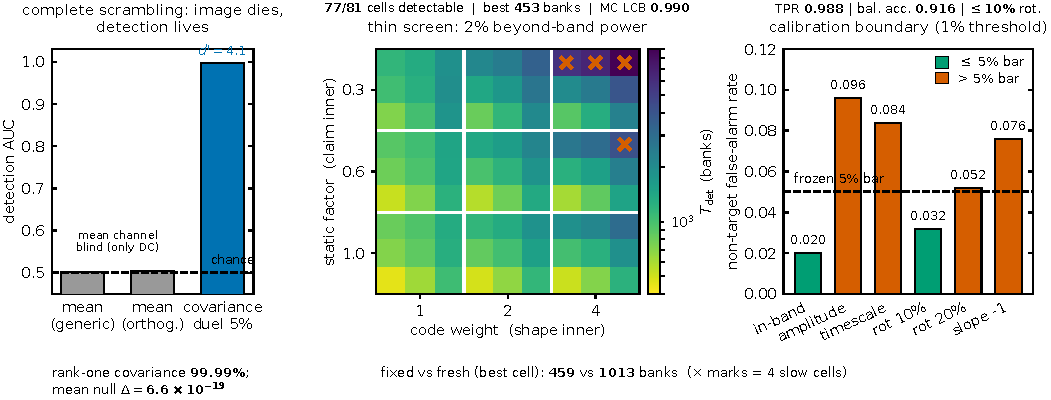
\includegraphics[width=\textwidth]{fig3_optical_realizations.pdf}
\caption{\textbf{Two optical endpoints and the honest boundary.} \emph{Left:} the
sealed thin-screen detector meets its $2\%$ beyond-band power endpoint in
$77/81$ predeclared cells, best cell $453$ banks, Monte Carlo power lower bound
$0.990$, with a fixed-versus-fresh latency advantage of $459$ versus $1013$
banks. \emph{Center:} at the frozen $1\%$ alarm threshold, four-class balanced
accuracy is $0.916$ and in-band false alarms are $0.020$, but medium-amplitude
and medium-timescale events give false-alarm rates of $0.096$ and $0.084$, and
robustness is frozen to the $\le10\%$ aperture-rotation domain; these are the
measured attribution limits, not fine print. \emph{Right:} at the complete-scramble
endpoint the mean channel is at chance while the covariance duel reaches $d'=4.1$,
$\mathrm{AUC}=0.997$ for a generic $5\%$ change, with rank-one covariance
($99.99\%$) and mean null $6.6\times10^{-19}$.}
\label{fig:optics}
\end{figure*}

\section*{Sealed optical instantiation}
A preregistered thin-screen experiment on a true single-pixel bucket record
converts the theorem into a power-certified sentinel. Under the sealed protocol
(End Matter~C), $2\%$ beyond-band changes were predicted detectable in $77/81$
cells; the best cell required $453$ banks and achieved a Monte Carlo power lower
bound of $0.990$; a repeated code bank retained a latency advantage of $459$
versus $1013$ banks over fresh covariance codes; and online scoring consumed
$0.16\%$ of each bank interval. This is a power-certified beyond-band alarm with
measured attribution leakage, not a fully specific sentinel: at the frozen $1\%$
threshold the four-class balanced accuracy was $0.916$ and in-band false alarms
were $0.020$, while medium-amplitude and medium-timescale events produced
false-alarm rates of $0.096$ and $0.084$ (Fig.~\ref{fig:optics}). For robustness,
all frozen performance and calibration bars passed in the primary mismatch domain
of aperture-preserving medium-basis rotations up to $10\%$ ($\mathrm{FA}=0.032$,
latency inflation $19\%$). At $20\%$ rotation and a spectral-slope mismatch of
$-1$, non-target false alarms rose to $0.052$ and $0.076$; these points define the
measured robustness boundary, and no broader law-mismatch claim is made.

% ---------------------------------------------------------------------
% CONCLUSION  (0.20 pp)
% ---------------------------------------------------------------------
\section*{Outlook}
Identifiability dimension can vanish while local hypothesis distinguishability
remains complete at a higher contact order. This invites classifying a
statistical sensing experiment by three independent objects---its
\emph{support} (where the law can respond), its \emph{rank} (how many scene
coordinates it reconstructs), and its \emph{jet} (the contact order at which a
chosen direction becomes observable). Strong disorder can enlarge support,
decrease rank, and leave jet order finite; no single scalar information budget
captures this Disorder Observability Triangle, whose first physical realization
is Fig.~\ref{fig:hero}. A clean positive corollary bounds the honest scope: on the
monotone cone ($x\ge0$, $\delta\ge0$, $G$ entrywise nonnegative and $G\succ0$),
$Q(x+\delta)-Q(x)>0$ for every $\delta\neq0$, so local completeness becomes global
for physically monotone addition processes such as deposition, coating growth, and
damage accumulation. The result separates reconstruction dimension from
observability order and transfers beyond optics to disordered
sensing~\cite{LeeStone}, sequential change detection~\cite{Snieder}, singular
statistical models where finite-sample spectral emergence sets a second
threshold~\cite{BBP}, and quantum-inspired superresolution~\cite{Tsang}.

\begin{acknowledgments}
[FUNDING/ACKNOWLEDGMENTS]
\end{acknowledgments}

% =====================================================================
%  END MATTER  (up to two pages; specialist material)
% =====================================================================
\clearpage
\onecolumngrid
\begin{center}\textbf{\large End Matter}\end{center}
\twocolumngrid

% ------- A -------
\section*{Appendix A: Proof of Rank--Jet Separation and the quadratic specialization}
Let $P_x=P_{q(x),\eta}$ with $q:\mathbb{R}^N\!\to\mathbb{R}^r$ smooth and every
nuisance $\eta$ profiled. By the chain rule the efficient scene score is
$Dq_x^{\!\top}s_q$, where $s_q$ is the efficient score in functional space, so the
scene Fisher matrix is $I_x=Dq_x^{\!\top}J_q\,Dq_x$ with $J_q=\mathbb{E}[s_q
s_q^{\!\top}]$. Since $J_q\in\mathbb{R}^{r\times r}$, $\rank(I_x)\le\rank(Dq_x)\le
r$, which is Eq.~\eqref{eq:rank}. Rank is therefore controlled by the number of
scene functionals the law exposes and is independent of sample size.

For the contact order, expand the profiled Chernoff distance along $\delta$. Write
$q(x+\eps\delta)-q(x)=\eps\,u(\delta)+\tfrac{\eps^2}{2}v(\delta)+o(\eps^2)$ with
$u,v$ projected off the nuisance tangent. For a regular reduced law
$\Cstar(\eps;\delta)$ is analytic in the functional displacement and vanishes to
second order in it, so if $u\neq0$ then
$\Cstar=c_1\eps^2+o(\eps^2)$ and $m=1$; if $u=0$ but $v\neq0$ then
$\Cstar=c_2\eps^4+o(\eps^4)$ and $m=2$. Equation~\eqref{eq:jet} then gives
$\Treq\asymp\eps^{-2m}$.

Specialize to the Gaussian covariance law $\Sigma(x)=\Sigma_0+z(\eps)H$,
$\Sigma_0\succ0$, with $K=\Sigma_0^{-1/2}H\Sigma_0^{-1/2}$. The exact divergences
are $D(P_\eps\|P_0)=\tfrac12[\tr A-\log\det(I+A)]=z^2\|K\|_F^2/4+O(z^3)$ and, at
the symmetric Chernoff point $s=\tfrac12$, $C=z^2\|K\|_F^2/16+O(z^3)$, with
$A=z K$. For the scrambled functional $Q(x)=x^{\!\top}Gx$, $G\succ0$, along
$x_\eps=x+\eps\delta$ the covariance shift is $z(\eps)=2c\,\eps+d\,\eps^2$ with
$c=x^{\!\top}G\delta$ and $d=\delta^{\!\top}G\delta>0$. If $c\neq0$ then
$z=2c\eps+O(\eps^2)$, so $C=c^2\|K\|_F^2\eps^2/4+o(\eps^2)$ and $m=1$. If $c=0$
then $z=d\eps^2$, so $C=d^2\|K\|_F^2\eps^4/16+o(\eps^4)$ and $m=2$: the ordinary
score vanishes, but the Hessian of $Q$ is $2G\succ0$, so the law leaves the null
at second order in every nonzero first-order-orthogonal direction. Because
$d>0$ for all $\delta\neq0$, no in-aperture direction is blind, establishing
Eq.~\eqref{eq:classes} and the empty blind set. \hfill$\square$

% ------- B -------
\section*{Appendix B: Nuisance quotient, amplitude-gauge collapse, and the minimal anchor}
Nuisance profiling is a projection in the Gaussian covariance Hilbert space with
inner product $\langle A,B\rangle_0=\tfrac12\tr(\Sigma_0^{-1}A\,\Sigma_0^{-1}B)$.
Collecting the nuisance covariance derivatives as columns $D_\eta$ and writing
$\Pi_\eta$ for the projector onto their whitened span, the efficient signal
direction is $H_\perp=(I-\Pi_\eta)H$ and $K$ is replaced by
$K_\perp=\Sigma_0^{-1/2}H_\perp\Sigma_0^{-1/2}$; all contact-order coefficients
carry $\|K_\perp\|_F$. If $H_\perp=0$ the change is unidentifiable from that
ledger.

The amplitude gauge is exactly this degeneracy. With an unknown medium amplitude
$a$, $\Sigma=R+a\,Q(x)H$, so $\partial_a\Sigma=QH$ and $\partial_Q\Sigma=aH$ are
collinear: zero-lag covariance carries \emph{zero} efficient information for
separating the scene functional $Q$ from $a$. The numerics confirm the collapse
to machine zero, both at zero lag and across proportional lags. Restoration
requires a signature outside the amplitude tangent: a second grain
kernel/wavelength or an independently normalized amplitude anchor. A finite
amplitude prior recovered $20\%$ of the naive information, and a second grain
kernel recovered a smaller finite fraction---the minimal anchor turns a hidden
fatal gauge into a design condition, shown as the amplitude-anchor icon in
Fig.~\ref{fig:hero}. This is the exact content of boundary~2 of the theorem.

% ------- C -------
\section*{Appendix C: Model/protocol capsule and integrity disclosures}
\emph{Theorem exams.} The jet and scrambling tests use the exact Kronecker
speckle generator (fully developed circular-complex-Gaussian field, factorized
grain$\otimes$code covariance) on a $32\times32$ grid, $N=1024$, code band
$P_B=3$, grain band $K=13$, $M=36$ codes, $10^4$ photons per bucket, and perform
no reconstruction.

\emph{Sealed detector.} The thin-screen sentinel uses a true zero-dimensional
bucket record on a $64\times64$ scene ($N=4096$), modulator band $k_p=5$, $M=128$
signed effective codes realized by $256$ complementary nonnegative exposures per
bank at a $20\,\mathrm{kHz}$ pattern rate ($12.8\,\mathrm{ms}$ per bank, cap
$T_{\mathrm{eff}}=4096$ banks $=52.4\,\mathrm{s}$), $10^4$ detected
photoelectrons per physical bucket, and a quasi-static medium within a bank that
is independent between banks. Every engine uses the physical
complementary-exposure shot term $|P|x$; the signed-difference mean is never used
as photon throughput. The sealed run used $12$ confirmatory banks and
$2.76$ of a $6.0$ GPU-hour ceiling. Thresholds were committed before confirmatory
generation, and no scene, code, medium realization, anomaly, or seed crosses
banks; there was one sealed run and no repair.

\emph{Integrity disclosure 1 (record generator).} After protocol freeze and
before unblinding, the record generator was refactored solely to stream Monte
Carlo records in GPU-memory chunks; an audited diff found no changes to
hypotheses, thresholds, bank counts, scenes, estimators, or endpoints, although
altered random-number consumption produced a different, still-blinded realization
set. All reported decisions apply the frozen analysis unchanged to that disclosed
chunked stream.

\emph{Integrity disclosure 2 (shot model).} A mandated independent-engine check
exposed a signed-code shot-noise error that had inflated covariance Fisher
information by approximately $1.9\times$; replacing the signed difference $Px$
with the physical complementary-exposure throughput $|P|x$ reduced the frozen
$P1$ witness coverage from $0.050$ to $0.033$ and eliminated the apparent
natural-scene living pocket, so all values reported here come from the corrected
artifacts and every prior kill only strengthened.

% =====================================================================
%  REFERENCES
% =====================================================================
\begin{thebibliography}{99}

\bibitem{FengMemory}
S. Feng, C. Kane, P.~A. Lee, and A.~D. Stone,
Correlations and fluctuations of coherent wave transmission through disordered
media, Phys. Rev. Lett. \textbf{61}, 834 (1988).

\bibitem{LeeStone}
P.~A. Lee and A.~D. Stone,
Universal conductance fluctuations in metals, Phys. Rev. Lett. \textbf{55}, 1622
(1985).

\bibitem{Tsang}
M. Tsang, R. Nair, and X.-M. Lu,
Quantum theory of superresolution for two incoherent optical point sources,
Phys. Rev. X \textbf{6}, 031033 (2016).

\bibitem{Mudry}
E. Mudry \textit{et al.},
Structured illumination microscopy using unknown speckle patterns,
Nat. Photonics \textbf{6}, 312 (2012).

\bibitem{Idier}
J. Idier \textit{et al.},
On the superresolution capacity of imagers using unknown speckle illuminations,
IEEE Trans. Comput. Imaging \textbf{4}, 87 (2018).

\bibitem{Chaigne}
T. Chaigne \textit{et al.},
Super-resolution photoacoustic fluctuation imaging with multiple speckle
illumination, Optica \textbf{3}, 54 (2016).

\bibitem{Snieder}
R. Snieder, A. Gr\^et, H. Douma, and J. Scales,
Coda wave interferometry for estimating nonlinear behavior in seismic velocity,
Science \textbf{295}, 2253 (2002).

\bibitem{Dechant}
A. Dechant and S.-i. Sasa,
Fluctuation-response inequality out of equilibrium,
Proc. Natl. Acad. Sci. U.S.A. \textbf{117}, 6430 (2020).

\bibitem{Lorden}
G. Lorden,
Procedures for reacting to a change in distribution,
Ann. Math. Statist. \textbf{42}, 1897 (1971).

\bibitem{HermannKrener}
R. Hermann and A.~J. Krener,
Nonlinear controllability and observability,
IEEE Trans. Autom. Control \textbf{22}, 728 (1977).

\bibitem{BBP}
J. Baik, G. Ben Arous, and S. P\'ech\'e,
Phase transition of the largest eigenvalue for nonnull complex sample covariance
matrices, Ann. Probab. \textbf{33}, 1643 (2005).

\end{thebibliography}

\end{document}
